\section {Linux哲学}
\begin{frame}{Linux哲学}
\pause
\begin{center}
\tikz[align=center]\node[draw,line width=6pt,rounded corners=8pt,inner sep=5mm] {\fontsize{35}{35}\selectfont K.I.S.S. \\ \\ \fontsize{20}{20}\selectfont Keep It Simple,Stupid};

\end{center}
\end{frame}


\begin{frame}{无名师的Linux心传}
\begin{center}
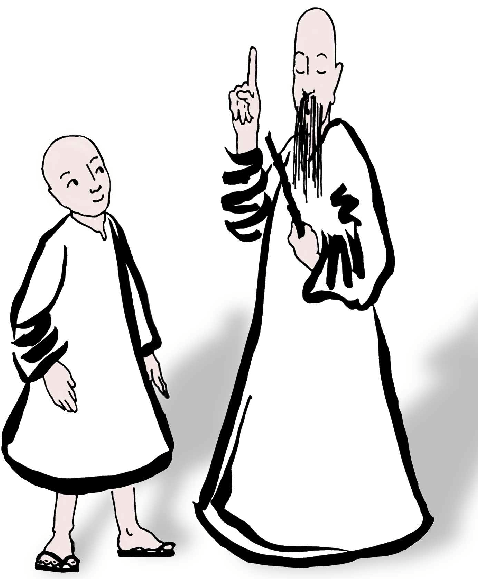
\includegraphics[height=0.7\textheight]{images/zen-linux.png} 
\end{center}
\end{frame}

\begin{frame}[shrink=5]{无名师与最终用户}
无名师又一次布道时,一个最终用户听说了他的智慧,跑来求 教。 他对无名师三鞠躬。\\
“我欲学习Unix大道,”他说,“但是弄不 懂命令行。”\\
 一个旁观的新门徒开始嘲讽最终用户,说他脑子一锅粥,说只有 训练有素、有智慧者才配适用Unix。 无名师抚手不语,命这个嘲笑最终用户的新门徒前坐,坐到最终 用户身边。 \\
 “告诉我,”他对新门徒说,“你写过什么代码,有过什么突出 设计。”\\
新门徒嗫嚅了两句,然后沉默了。 无名师转向最终用户。“告诉我”,他问,“为何你要寻求大 道?”\\
“我用的软件并不能令我满意”,最终用户答,“既不稳定,也 不美观。听说Unix之道尽管艰难,但超越一切,我愿抛去一切诱 饵和虚像。” \\
“那么,”无名师问,“你为何想尽办法让软件帮你做事?” \\
“我是一个建筑工”,最终用户答道,“这座城里的很多房屋都 出自我手。” \\
无名师转向新门徒。“家猫也能欺负老虎”,无名师说,“但是 猫叫永远比不过虎吼。” \\
听到此,新门徒眼中一亮。
\end{frame}

\begin{frame}[shrink]{无名师与Unix狂}
一个Unix狂热者听说无名师掌握Unix大道真理,便跑来求教。无 名师对他说: \\
“ 当尊者Thompson发明Unix时,他并不理解它。随后他理解了,受 益了,不再发明了。”  \\
“当尊者McIlroy发明管道时,他只知道他将传递软件,并不知 道他能传播思想。” \\
“当尊者Ritchie发明C时,他将程序员放到缓冲区溢出、堆损坏 和烂指针bug的地狱中惩罚。”\\
“说实话,这些尊者既瞎由蠢!” 狂热者堆无名师的用词极为愤怒。\\
 “这些智者”,他抗议到,“给了我们Unix的大道。我们嘲笑他 们,就是混淆是非,比转世为畜生和MCSE害不如。”\\
  “你的代码全无污点和缺陷?”无名师问。\\
   “不”,狂热者承认,“没人不犯错。”\\
   “这些尊者之智,”无名师说,“就是了解自身之愚。” 听到此,狂热者眼中一亮。
\end{frame}

\begin{frame}[allowframebreaks,allowdisplaybreaks]{无名师与脚本狂}
无名师和学生吃早饭时,从黑客大陆来了一个陌生访客。\\
 “I hear y00 are very 133t,”,他说。“P133z teach m3 all y00 know”。(我听说你很牛,请把你会的都教给我。) 无名师的学生面面相觑,都没有听懂这类粗鄙言语。\\
 无名师微笑 道:“你想弄懂Unix?” \\
 “I want to b3 a wizard hax0r”,陌生人回答,“and 0wn ever3one’s b0xen。”(我想当个顶尖黑客,能掌握所有人的 机器。) \\
 “我不教这个”,无名师答道。\\
  陌生人很激动。“D00d,y00r nothing but p0ser”,他说“If y00 m00 anything,y00 wud t33ch m3.”(哥们儿,感情你没 真本事呀,你要知道点儿东西就教给我了。) \\
  “有条路。”无名师说,“可以将你带入真知。”他在纸上写了 个IP地址。“黑掉这台机器,这对你来说应该不费什么力气,他 的管理员不称职。回来我告诉我你发现了什么。”\\
   陌生人鞠了一躬机离开了。无名师把他的早饭吃完。\\
    几天过去了,几个月过去了。每人再想起陌生人。\\
     数年过去了,黑客大陆来的陌生人回来了。 \\
     “你混蛋!”他说,“我黑掉了那台机器,你说的没错,太容易 了,但是我被FBI抓起来扔进监狱了。”\\
      “好”,无名师说,“你可以继续下一课了。”他在另一张纸上 写了个IP地址交给陌生人。 \\
      “你疯了?”陌生人喊道,“经过这事,我再也不黑别人的机器 了。”\\
       无名师脸露微笑。“这里就是”,他说,“真知的开始。”\\
        听到此,陌生人眼中一亮。
\end{frame}